\documentclass{report}

\usepackage{amsmath}
\usepackage{amssymb}
\usepackage{graphicx}
\usepackage{helvet}

\setlength{\paperheight}{3in}
\setlength{\paperwidth}{4in}
\pdfpagewidth=\paperwidth
\pdfpageheight=\paperheight

\setlength{\textwidth}{3.5in}
\setlength{\textheight}{2.5in}

\setlength{\oddsidemargin}{-0.75in}
\setlength{\evensidemargin}{-0.75in}
\setlength{\topmargin}{-1.25in}

\newcommand{\sld}[1]{\newpage{\noindent\Large \underline{#1}}\vspace*{8pt}}
\newcommand{\itm}[1]{\vspace*{8pt}\noindent#1}
\newcommand{\itmb}{\itm{$\bullet$}\ }

\newcounter{gmlrx}
\newcounter{gmlry}
\newcommand{\gmnode}[3]{\put(#1,#2){\circle{20}}\put(#1,#2){\makebox(0,0){$#3$}}}
\newcommand{\gmplate}[5]{
\setcounter{gmlrx}{#1}\addtocounter{gmlrx}{#3}
\setcounter{gmlry}{#2}\addtocounter{gmlry}{-#4}
\put(#1,#2){\line(1,0){#3}}
\put(#1,#2){\line(0,-1){#4}}
\put(\value{gmlrx},\value{gmlry}){\line(-1,0){#3}}
\put(\value{gmlrx},\value{gmlry}){\line(0,1){#4}}
\setcounter{gmlrx}{#1}\addtocounter{gmlrx}{5}
\setcounter{gmlry}{#2}\addtocounter{gmlry}{-6}
\put(\value{gmlrx},\value{gmlry}){\makebox(0,0){$#5$}}
}



\begin{document}
\sf%
\vspace*{1pt}
\noindent
{\huge Ground Truth, \\[4pt] 
Machine Learning, \\[4pt]
{\sf and the} \\[8pt]
Mechanical Turk}
\\[24pt]
{\Large Bob Carpenter}
(w.\ Emily Jamison, Breck Baldwin)
\\[4pt]
{\large\emph{Alias-i, Inc.}}



\sld{Supervised Machine Learning}

\begin{enumerate}
\item Define coding standard mapping inputs to outputs, e.g.:
\begin{itemize}
\item English word $\rightarrow$ stem
\item newswire text $\rightarrow$ person name spans
\item biomedical text $\rightarrow$ genes mentioned
\end{itemize}
\item Collect inputs and code ``gold standard'' training data
\item Develop and train statistical model using data
\item Apply to unseen inputs
\end{enumerate}



\sld{Annotation Bottleneck}

\begin{itemize}
\item Bottleneck is collecting training corpus
\item Commericial data's expensive (e.g.\ LDA, ELRA)
\item Academic corpora typically restrictively licensed
\item Limited to existing corpora
\item For new problems, use:
self, grad students, temps, interns, \ldots
\vspace*{12pt}
\item Mechanical Turk to the rescue
\end{itemize}


\sld{Example: Named Entities}

\hspace*{-24pt}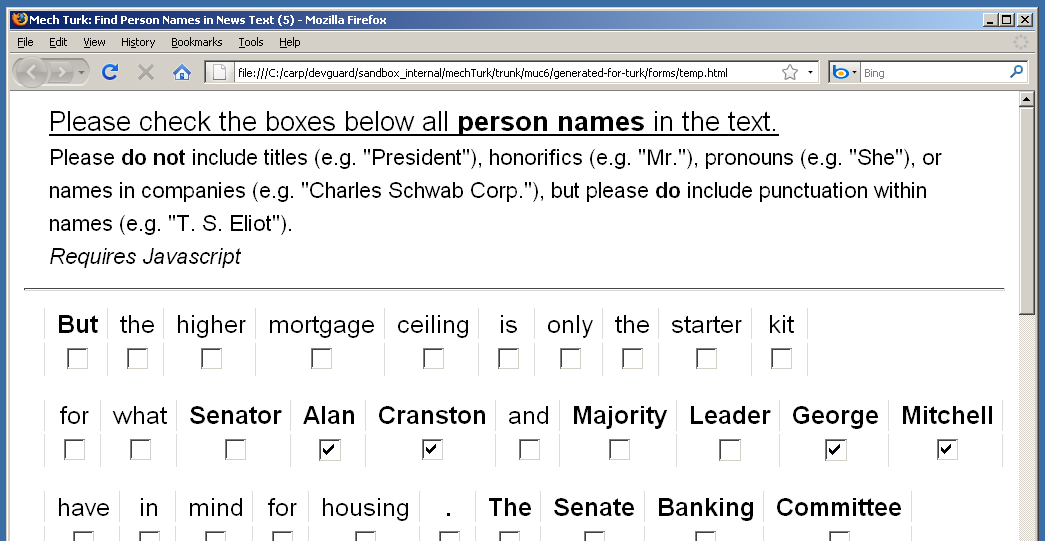
\includegraphics[width=1.05\textwidth]{pngs/big-ne-form.png}


\sld{Discussion: Named Entities}

\begin{itemize}
\item Conveying the coding standard
\begin{itemize}
\item Official MUC-6 standard dozens of pages
\item Examples are key
\item (Maybe a qualifying exam)
\end{itemize}

\item User Interface Problem
\begin{itemize}
\item One entity type at a time (vs. pulldown menus)
\item Checkboxes (vs. highlighting spans)
\end{itemize}
\end{itemize}

\sld{Discussion: Named Entities (the good)}

\begin{itemize}
\item 190K tokens, 64K capitalized, 4K names
\item Less than a week at 2 cents/400 tokens
\item Turkers overall better than LDC data
\begin{itemize}
\item Correctly Rejected:
{\tt\footnotesize Webster's, Seagram, Du Pont, Buick-Cadillac, Moon, erstwhile Phineas Foggs}
\item Incorrectly Accepted: {\tt\footnotesize Tass}
\item Missed Punctuation: {\tt\footnotesize J~E.~``Buster'' Brown}
\end{itemize}
\item Many Turkers no better than chance \\
(c.f.\ social psych by Yochai Benkler, Harvard)
\end{itemize}


\sld{Morphological Stemming}

\hspace*{-24pt}
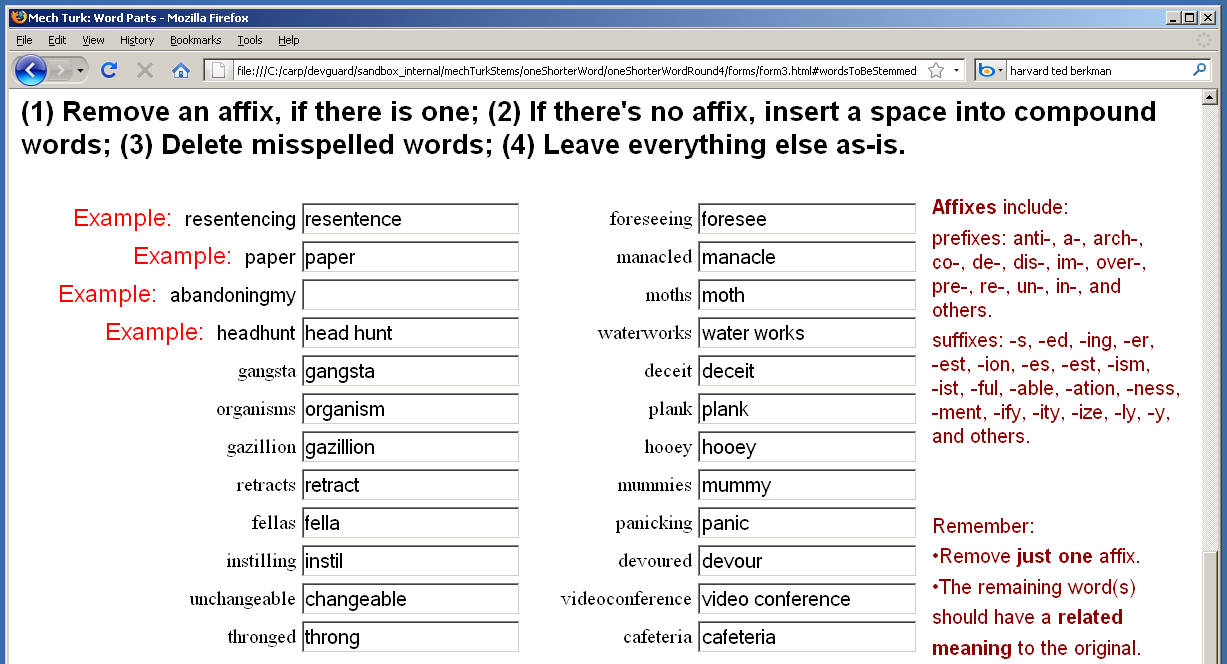
\includegraphics[width=1.05\textwidth]{pngs/stems-v4.png}


\sld{Instructions plus Qualifying Test}

\begin{itemize}

\item Four rounds of annotation

\item Simplified task to one stem

\item Added instructions with detailed examples

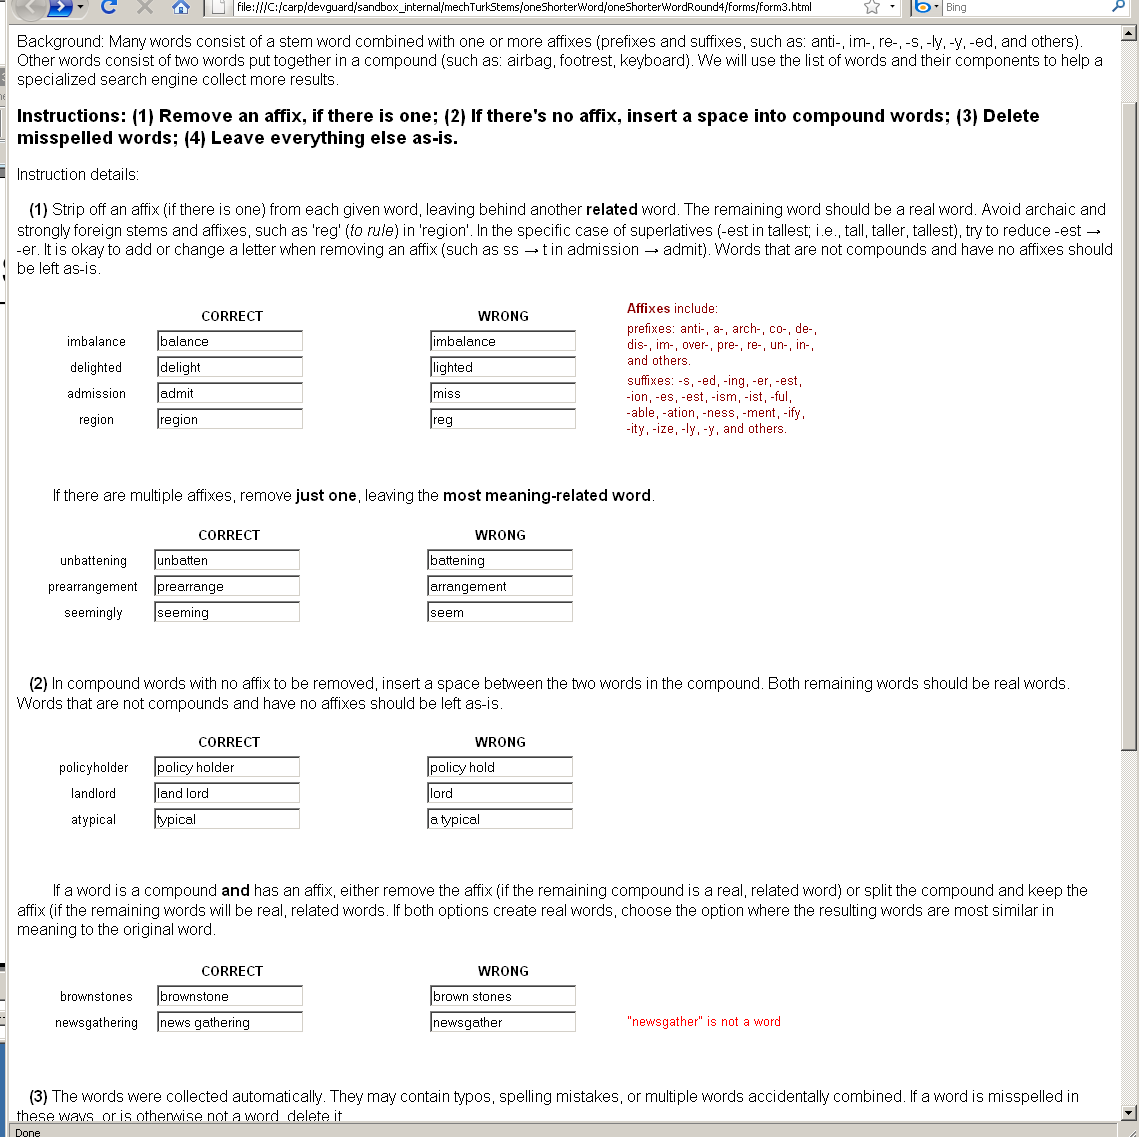
\includegraphics[width=0.2\textwidth]{pngs/stems-instrux.png}

\item Added qualifying test 

\end{itemize}



\sld{Gene Linkage HIT}

\hspace*{-24pt}
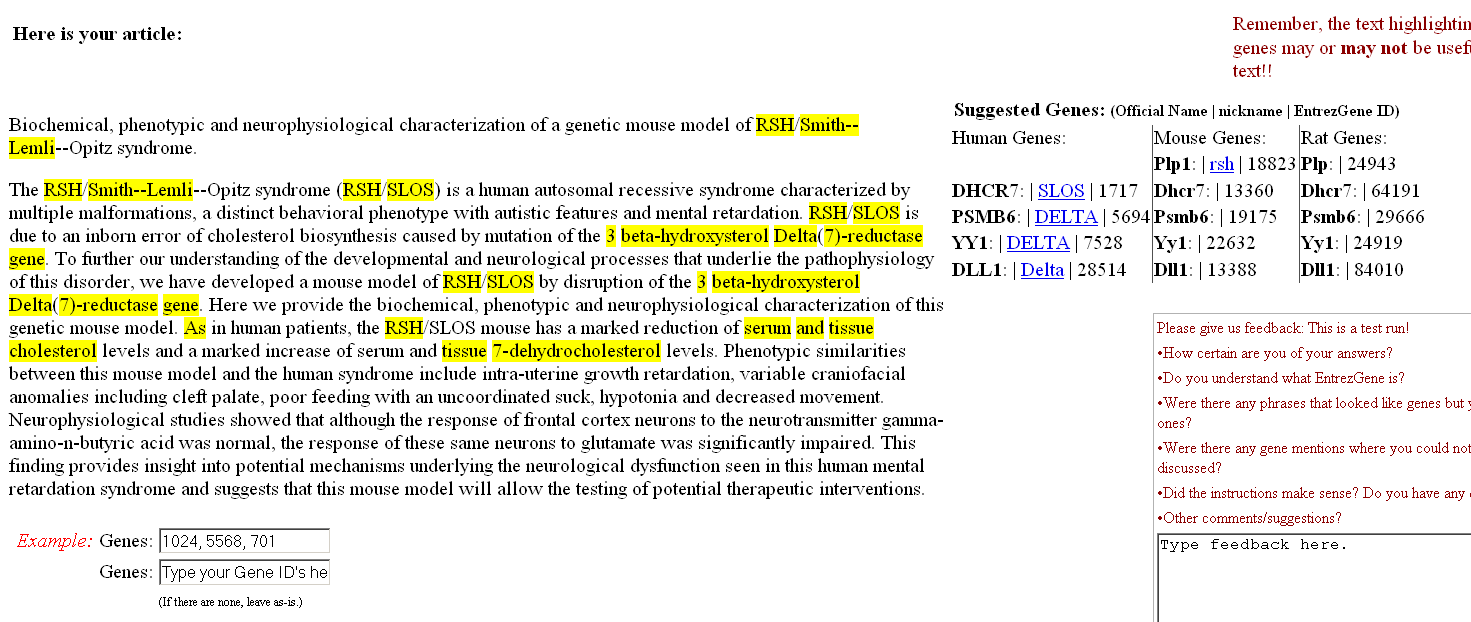
\includegraphics[width=1.05\textwidth]{pngs/gene-task.png}

\sld{Text to Gene Linkage Failed}


\begin{itemize}
\item This is what we really care about
\item Paid for by NIH grant
\item Could get them to pass qualifier
\item Could not get Turkers to take task even at \$1/hit
\vspace*{12pt}
\item Are complex, specialized tasks like this possible?
\end{itemize}


\sld{Voted Gold Standard}

\begin{itemize}
\item Turkers vote
\item Label with majority category
\item Censor if no majority
\end{itemize}


\sld{Some Labeled Data}

\begin{itemize}
\item Seed the data with cases with known labels
\item Performance on known cases estimates annotator accuracy
\item Vote with adjustment for accuracy
\vspace*{18pt}
\item Requires large amount of annotated data for:
\begin{itemize}
\item estimating accuracies well
\item liveness for new items
\end{itemize}
\end{itemize}


\sld{Estimate Everything (may use known)}

\begin{itemize}
\item Gold standard labels
\item Annotator accuracies
    \begin{itemize}
      \item sensitivity (false negative rate; misses)
      \item specificity (false positive rate; false alarms)
      \item imbalance indicates bias; high values accuracy
    \end{itemize}
\item Coding standard difficulty
    \begin{itemize}
        \item Average accuracies
        \item Variation among annotators
    \end{itemize}
\item Item difficulty (not enough data)
\end{itemize}


\sld{Beta-Binomial ``Random Effects''}


\begin{picture}(195,145)

\gmnode{57.5}{132.5}{\alpha_0}
\gmnode{97.5}{132.5}{\beta_0}
\gmnode{142.5}{132.5}{\alpha_1}
\gmnode{182.5}{132.5}{\beta_1}
\gmnode{77.5}{92.5}{\theta_{0,j}}
\gmnode{162.5}{92.5}{\theta_{1,j}}
\gmnode{10}{30}{\pi}
\gmnode{55}{30}{c_i}
\gmnode{120}{30}{x_k}

\put(57.5,122.5){\vector(1,-1){19.75}}  % alpha_0 to theta_0_j
\put(97.5,122.5){\vector(-1,-1){19.75}} % beta_0 to theta_0_j
\put(142.5,122.5){\vector(1,-1){19.75}}  % alpha_1 to theta_1_j
\put(182.5,122.5){\vector(-1,-1){19.75}} % beta_1 to theta_1_j
\put(20,30){\vector(1,0){25}}  % \pi to c_i
\put(65,30){\vector(1,0){45}}  % c_i to x_k
\put(77.5,82.5){\vector(1,-1){42.5}}  % theta_0_j to x_k
\put(162.5,82.5){\vector(-1,-1){42.5}}  % theta_1_j to x_k

\gmplate{30}{55}{50}{50}{I}
\gmplate{95}{55}{50}{50}{K}
\gmplate{45}{115}{150}{45}{J}

\end{picture}


\sld{Why we Need Task Difficulty}

\begin{itemize}
\item What's your estimate for:
\begin{itemize}
\item a baseball player who goes 12 for 20?
\item a market that goes down 9 out of 10 days?
\item \ldots
\end{itemize}
\item Must smooth annotators with few annotations (e.g. 20 labels)
\item Hierarchical model of accuracy prior does this
\end{itemize}


\sld{Hard vs. Soft Gold: Posterior Uncertainty}


\begin{itemize}
\item Some items are really marginal
\item Traditionally censored or added with false confidence
\vspace*{12pt}
\item Posterior uncertainty can be modeled
\end{itemize}


\sld{Posteriors for Dentistry Data Items}

\hspace*{-24pt}
\begin{tabular}{ll}
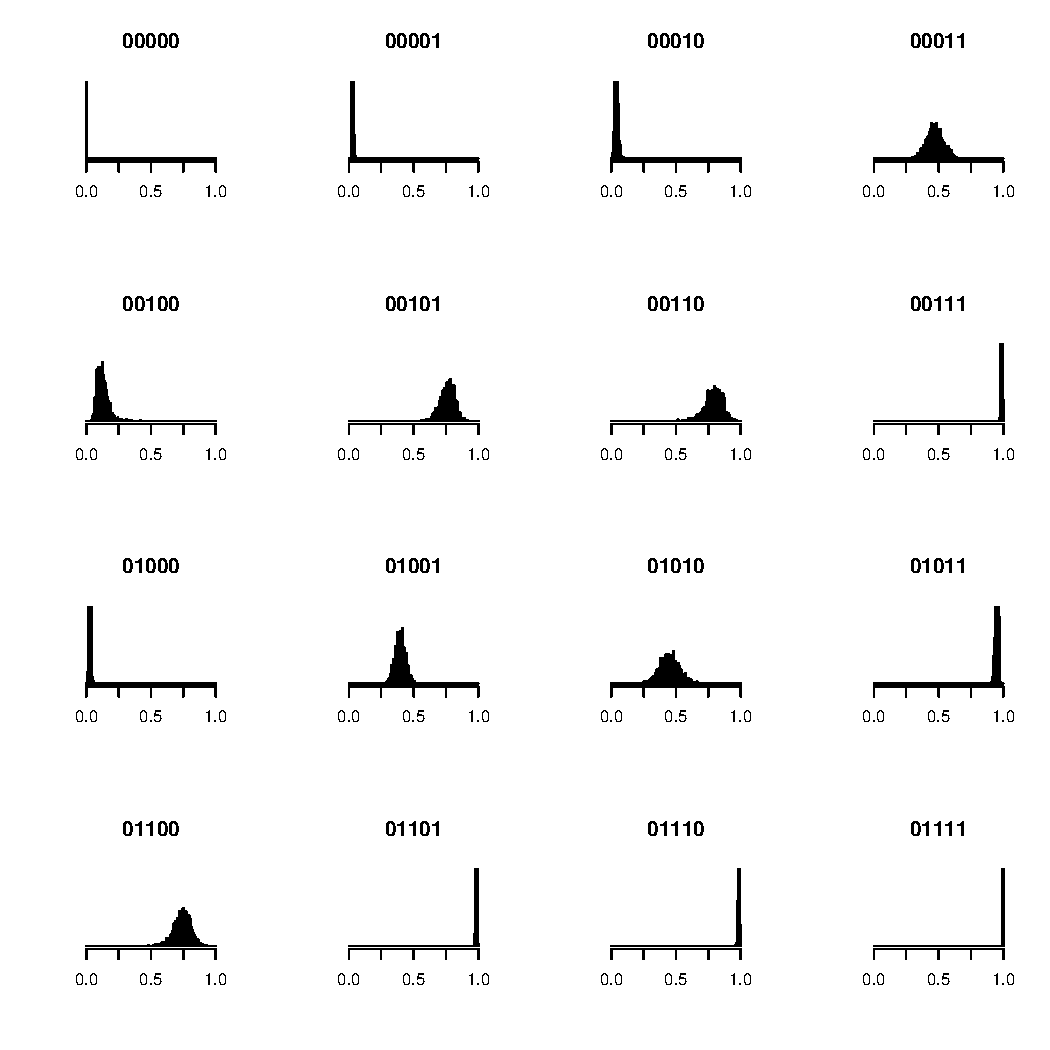
\includegraphics[width=0.5\textwidth]{pngs/model-4-cat-posteriors-dentistry.pdf}
&
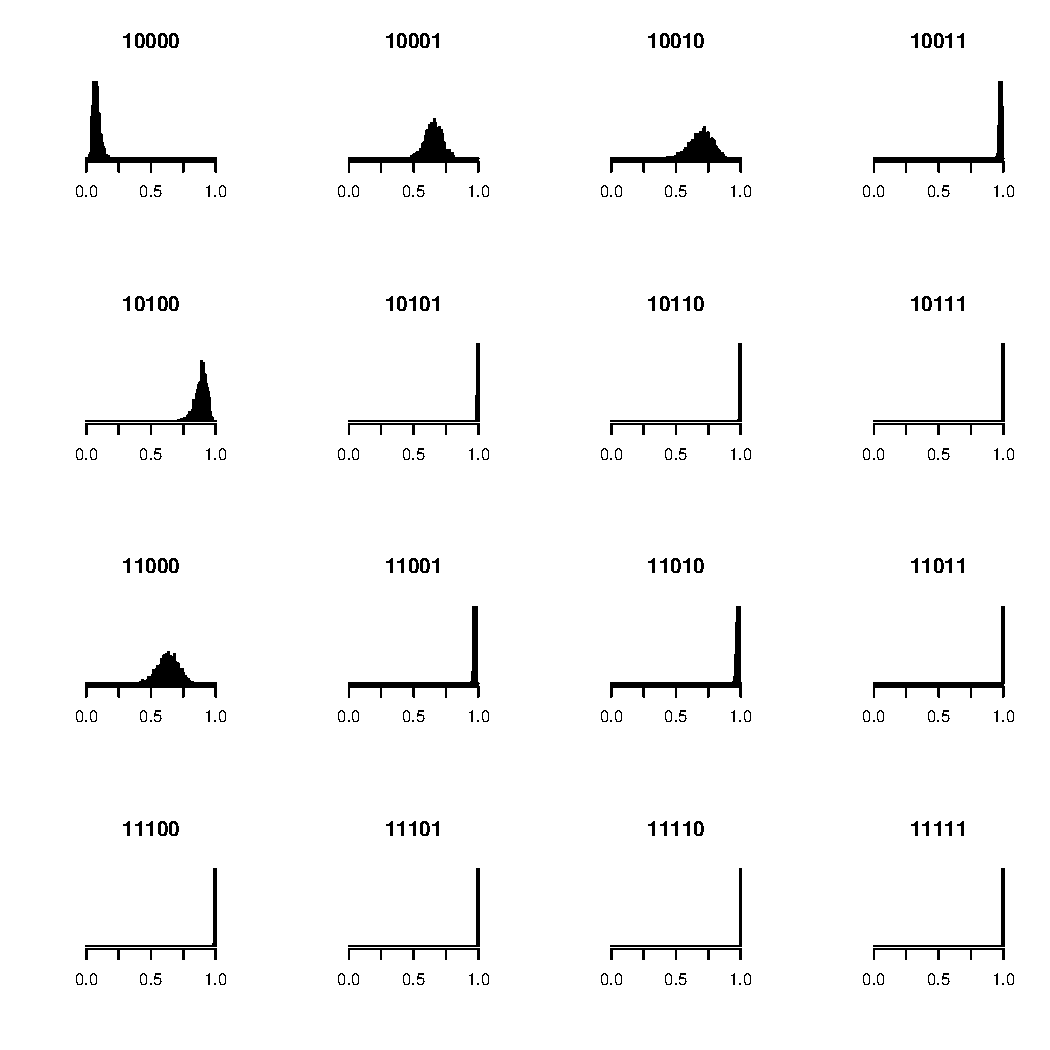
\includegraphics[width=0.5\textwidth]{pngs/model-4-cat-posteriors-dentistry-2.pdf}
\end{tabular}

Accounts for bias, so very different from simple vote!



\sld{Posteriors for Dentist Accuracies}

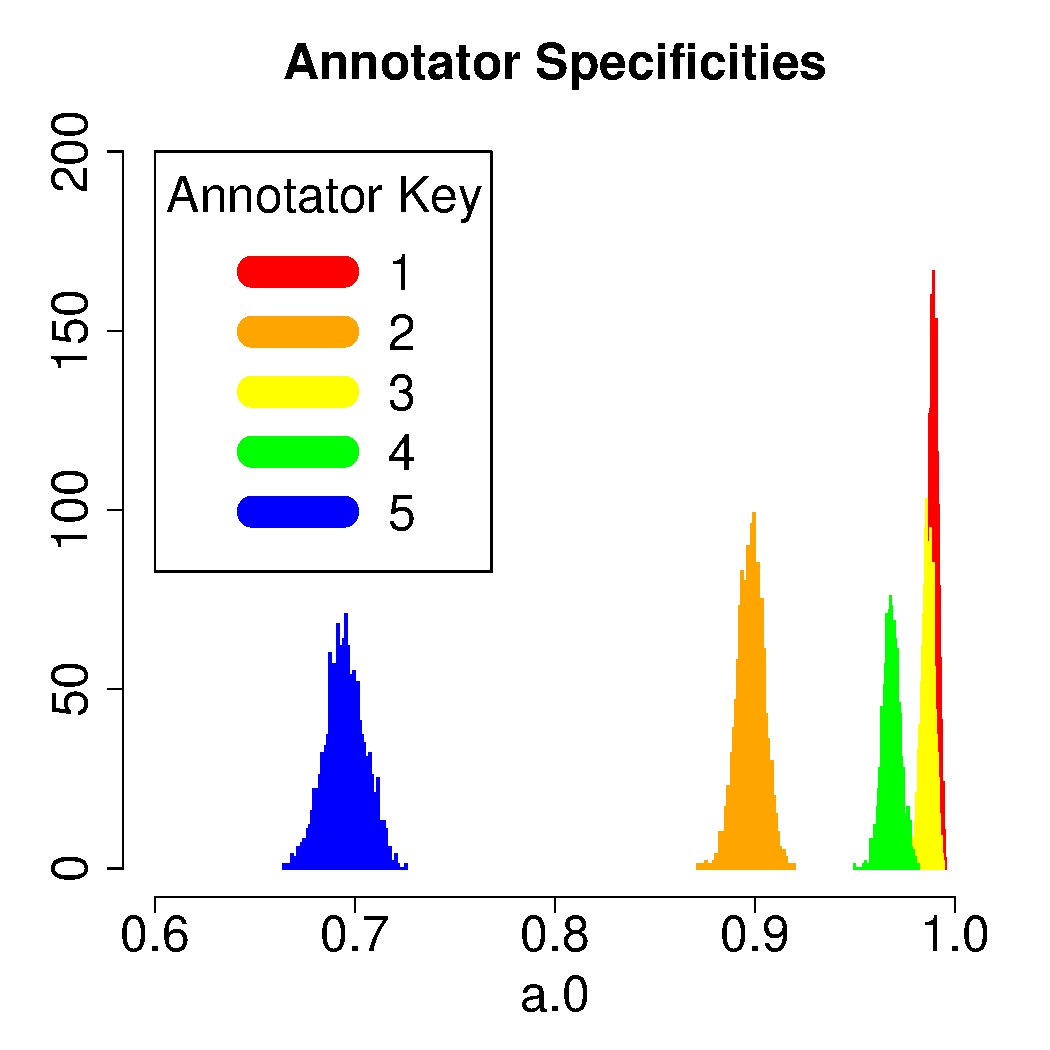
\includegraphics[width=0.4\textwidth]{pngs/a-0-hist.pdf}
\ \ \
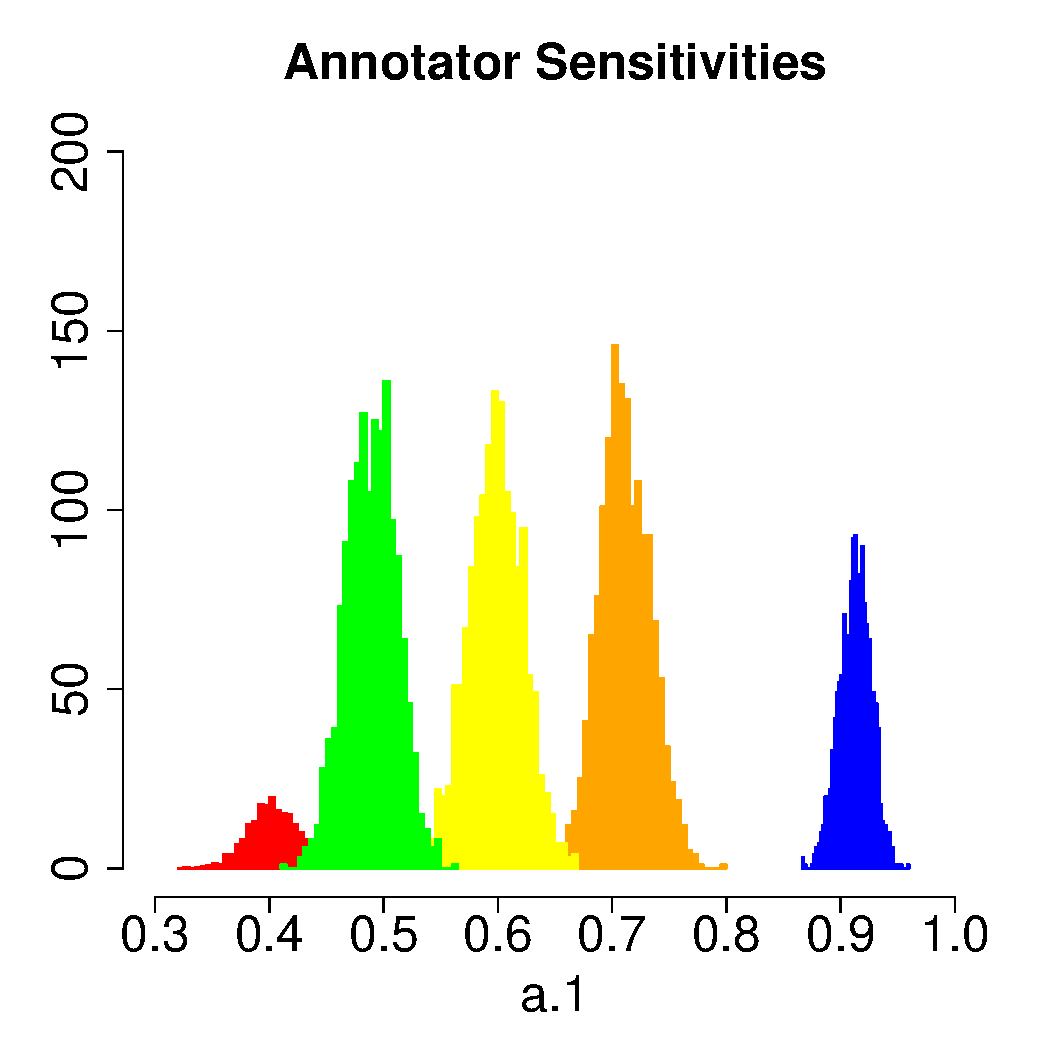
\includegraphics[width=0.4\textwidth]{pngs/a-1-hist.pdf}

\begin{itemize}
\item Posterior density vs. point estimates (e.g. mean)
\end{itemize}


\end{document}
